%
% fig-hauptwert.tex
%
% (c) 2026 Prof Dr Andreas Müller
%
\begin{figure}
\centering
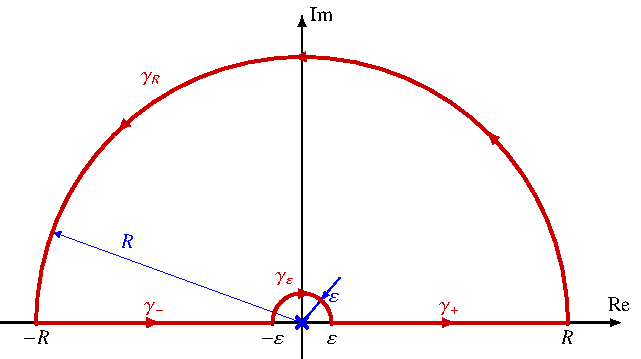
\includegraphics{chapters/030-integration/images/hauptwert.pdf}
\caption{Weg zur Berechnung des Integrals
\eqref{buch:integration:residuen:eqn:sinxxintegral}
mit Hilfe des Weges $\gamma$, der sich aus einem grossen
Kreis mit Radius $R$ und einem kleinen Kreis mit Radius
$\varepsilon$ zusammensetzt.
Dadurch wird die Singularität des Integranden $e^{iz}/z$ an der Stelle
$z=0$ gemieden.
\label{buch:integration:residuen:fig:hauptwert}}
\end{figure}
